\documentclass[main.tex]{subfiles}
\newcommand\chapterlabel{Ch-solutions}\setcounter{figurenewcounter}{0}\setcounter{tablenewcounter}{0}\setcounter{formulanewcounter}{0}


\begin{document}
\linenumbers
%\setcounter{chapter}{5}
  
\chapter[Physical properties of solutions]{Physical properties of solutions}
%\label{ch:atoms}


      \begin{marginfigure}
      \begin{tikzpicture} \node (a) at (0,0) {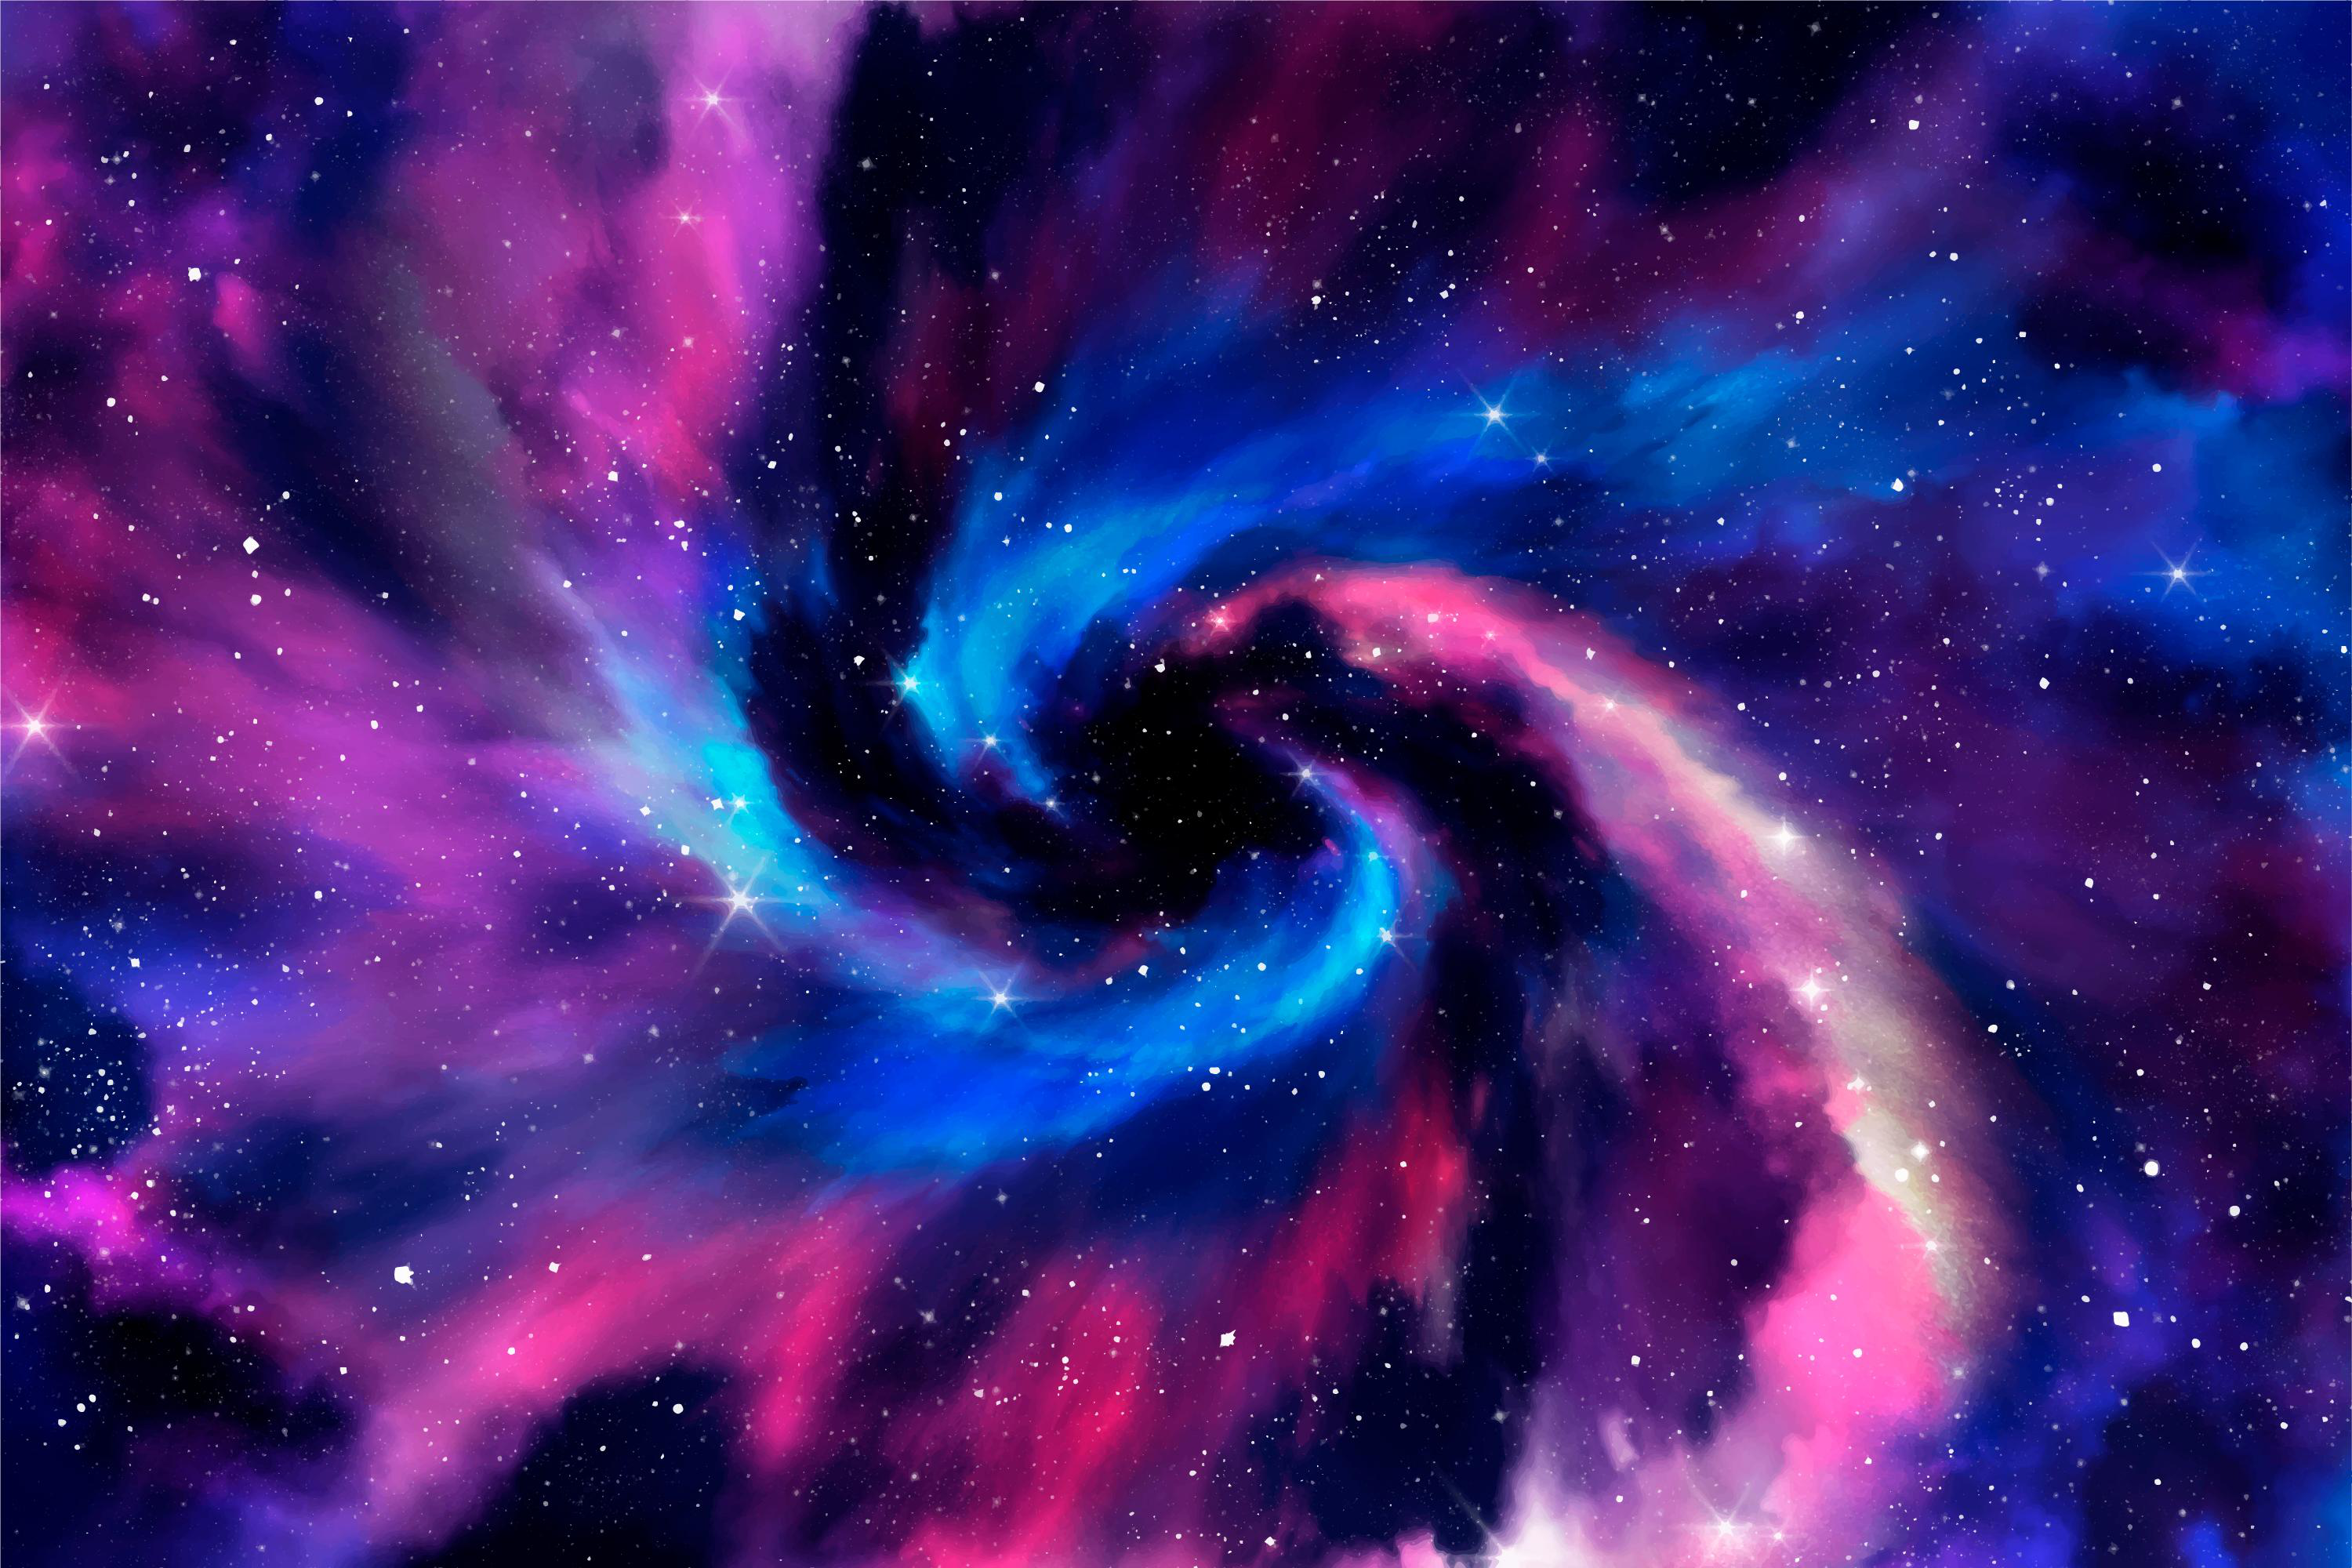
\includegraphics[width=4cm]{../Ch-solutions/figure1}} node[rotate=90, font=\tiny] at ([yshift=.5cm,xshift=.1cm]a.south east) {\textsuperscript{\textcopyright} PxFuel} ;
\end{tikzpicture}
\end{marginfigure}


\lettrine[lines=4]{\color{black!45}S}{olutions} are homogeneous mixtures of a solvent and one or more solutes. In your everyday life, you will encounter numerous liquid-based mixtures, from recovery drinks to fancy champagne or plain milk. However, solutions are not just liquid-based as you can also find solid solutions such as an alloy, and even gas solutions such as the air. This chapter will cover the physical properties of solutions--boiling, freezing, and melting--and in particular, we will gain insight into the impact of the solute on the physical properties of the solvent. The chapter will also address the meaning of different concentration units and the relationship between them, as well as the properties of colloids--a special type of unstable mixture. 
\begin{marginfigure}%LEARNING GOALS BOX
\begin{mytcbox}{GOALS}
\begin{enumerate}[label=\protect\circled{\color{white}\arabic*}]
\item Compute different concentration units
\item Interconvert concentration units
\item Predict freezing and boiling point of solutions
\item Predict the vapor pressure of solutions
\item Identify colloids
\end{enumerate}
\end{mytcbox}
\vspace{1cm}
\begin{tcolorbox}[enhanced,colback=red!5!white,colframe=black!50!red,boxrule=1pt,
  arc=0pt,outer arc=0pt,drop heavy lifted shadow]
\faGears\ 
\docenvdef{Discussion:} What does it means the term colligative, like in colligative properties of solutions? List four colligative properties of a solution.  \end{tcolorbox}
\end{marginfigure}%LEARNING GOALS BOX



\section{Solutions and colloids}
A solution is a homogeneous mixture of a solvent and one or more solutes. Homogeneous means that a solution consists of only one visible phase (e.g. wine) in contrast to heterogeneous which means that a mixture would be composed of two or more distinct phases (e.g. a chocolate chip cookie). 

\sloppy 
\begin{description}

\item[\docfilehook{Solutions in terms of phase and solubility}{}] 
One can find gas, liquid, or solid solutions depending on the final phase of the resulting solutions. For example, brass is a solid solution of copper and zinc and the air is a gaseous solution of oxygen, nitrogen, and other components. Solutions can be classified in terms of solubility. The solubility of a given solute in a solvent is the maximum amount of solute one can dissolve in a volume of solvent. Solutions can be saturated when they contain the maximum amount of solute one can fit, unsaturated when they contain less than the maximum amount of solute one can fit, or supersaturated when they contain more than a saturated solution. Supersaturated solutions tend to be unstable and the solute tends to eventually precipitate.
 \begin{center}
\refstepcounter{table}  \label{tab:{\chapterlabel}1}
\fontfamily{ppl}\selectfont
\begin{tabular}{llll}
\rowcolor{black!45}
\toprule
\multicolumn{4}{l}{\hypersetup{colorlinks,linkcolor={white}} \cellcolor{black}\color{white}\bfseries\small Table \ref{tab:{\chapterlabel}1} Types of solutions } \\
\midrule
 \rowcolor{gray!10} Solute & Solvent & Solution state & Example\\
\midrule
Gas	& \multicolumn{1}{c}{Gas}&\multicolumn{1}{c}{Gas} &\multicolumn{1}{c}{Air} \\ 
Gas	& \multicolumn{1}{c}{Liquid}&\multicolumn{1}{c}{Liquid} &\multicolumn{1}{c}{Club soda} \\ 
Gas	& \multicolumn{1}{c}{Solid}&\multicolumn{1}{c}{Solid} &\multicolumn{1}{c}{\ce{H2} in Pd} \\ 
Liquid	& \multicolumn{1}{c}{Liquid}&\multicolumn{1}{c}{Liquid} &\multicolumn{1}{c}{Acetone in water} \\ 
Liquid	& \multicolumn{1}{c}{Solid}&\multicolumn{1}{c}{Solid} &\multicolumn{1}{c}{Easy light charcoal  } \\ 
Solid	& \multicolumn{1}{c}{Liquid}&\multicolumn{1}{c}{Liquid} &\multicolumn{1}{c}{Saltwater  } \\ 
Solid	& \multicolumn{1}{c}{Solid}&\multicolumn{1}{c}{Solid} &\multicolumn{1}{c}{Brass  } \\ 
 \bottomrule
\end{tabular}\end{center} 
Table \ref{tab:{\chapterlabel}1} reports different types of solutions with examples.


\item[\docfilehook{Solutions}{}] 
In solutions, the solute particles are dispersed evenly throughout the solvent giving homogeneous mixtures. As such, in a solution such as seawater, the solute cannot be visually distinguished from the solvent. The mixture appears transparent even when it may have a certain color. The solute particles are that small that they can go through filters and membranes.

\item[\docfilehook{Suspensions}{}] Suspensions are heterogeneous mixtures. The particles of a suspension are so large that they can often be visually seen and they can be trapped using filters and membranes. Because of its weight, suspended particles tend to segregate and settle out on the bottom of suspensions. Examples of suspensions are antacid mixtures or liquid penicillin. 




\stepcounter{figurenewcounter}   \refstepcounter{figure}  \label{Fig:{\chapterlabel}\thefigurenewcounter}
%\caption{Classification of the matter}
\hspace{-5cm}\vspace{-0.5cm}
\begin{minipage}[b]{1.\linewidth}
\begin{center}
\resizebox{1.3\textwidth}{!}{
\begin{tikzpicture}
  [
    start chain=p going below,
    every on chain/.append style={etape},
    every join/.append style={line},
    node distance=1 and .85,
  ]
  {
    \node (a) [on chain, join] {Mixtures};
    {[start branch=l going below left] \node (b) [on chain] {Solutions};}
    {[start branch=r going below right] \node (c) [on chain] {Suspension}; }
      {[start branch=c going below ] \node (d) [on chain] {Colloids}; }


\path [line] (a.south) -- ([yshift=-.5cm]a.south) --  ([yshift=.5cm]b.north) --  (b.north); 
\path [line]  		  ([yshift=-.5cm]a.south) --  ([yshift=.5cm]c.north) --  (c.north); 
\path [line]  		  ([yshift=-.5cm]a.south)  --  (d.north); 



 \node (e) at ([yshift=-1.5cm]b.south) {\includegraphics[width=3cm]{../{\chapterlabel}/seawater}} node[rotate=90, font=\tiny] at ([yshift=.5cm,xshift=.1cm]e.south east) {\textsuperscript{\textcopyright} Flirk} ; \node[text width=3cm,font=\small] at ([yshift=-.5cm, xshift=.4cm]e.south){Seawater is a solution};

 \node (e) at ([yshift=-1.5cm]c.south) {\includegraphics[width=3cm]{../{\chapterlabel}/muddywater}} node[rotate=90, font=\tiny] at ([yshift=.5cm,xshift=.1cm]e.south east) {\textsuperscript{\textcopyright} Wallpaperflare} ; \node[text width=4cm,font=\small] at ([yshift=-.5cm, xshift=.4cm]e.south){Muddy water is a suspension};
  \node (f) at ([yshift=-1.6cm]d.south) {\includegraphics[width=3cm, height=2.9cm]{../{\chapterlabel}/milk}} node[rotate=90, font=\tiny] at ([yshift=.5cm,xshift=.1cm]f.south east) {\textsuperscript{\textcopyright} Flickr} ; \node[text width=3cm,font=\small] at ([yshift=-.2cm, xshift=.4cm]f.south){Milk is a colloid};
% 

  }
\end{tikzpicture}
}
\begin{tikzpicture}
 \node[text width=12cm, fontscale=.3,shift={(-0em,2em)}] at (0em,-0em) { \begin{bf}\color{black}\bfseries\large Figure \ref{Fig:{\chapterlabel}\thefigurenewcounter} \end{bf} Classification of the mixtures };
\end{tikzpicture}
\end{center}\end{minipage}


\begin{marginfigure}[9cm]
   \begin{tikzpicture} \node (a) at (0,0) {\includegraphics[width=4cm, height=4cm]{../{\chapterlabel}/tyndall1}} node[rotate=90, font=\tiny] at ([yshift=.5cm,xshift=.1cm]a.south east) {\textsuperscript{\textcopyright} www.wallpaperflare.com} ;
\node[text width=5cm] at ([yshift=0.6cm]a.north) {\mytriangle{red}The Tyndall effect of a liquid };
\end{tikzpicture}
%\begin{tikzpicture} \node (a) at (0,0) {\includegraphics[width=4cm, height=4cm]{../{\chapterlabel}/tyndall2}} node[rotate=90, font=\tiny] at ([yshift=.5cm,xshift=.1cm]a.south east) {\textsuperscript{\textcopyright} www.wallpaperflare.com} ;
%\node[text width=5cm] at ([yshift=0.6cm]a.north) {\mytriangle{red}The Tyndall effect};
%\end{tikzpicture}
\begin{tikzpicture} \node (a) at (0,0) {\includegraphics[width=4cm, height=4cm]{../{\chapterlabel}/tyndall3}} node[rotate=90, font=\tiny] at ([yshift=.5cm,xshift=.1cm]a.south east) {\textsuperscript{\textcopyright} wikipedia} ;
\node[text width=5cm] at ([yshift=0.6cm]a.north) {\mytriangle{red}The Tyndall effect of a gas};
\end{tikzpicture}
\end{marginfigure}

\item[\docfilehook{Colloids}{}] 
We have that solutions are homogeneous mixtures in the form of only one visible phase. If we add an ionic solute to a solvent, the solute particles would break down into ions and these ions would be solvated by the solvent molecules. As such,  the solute in solution exists in a different state than the solid solute. We also have that a heterogeneous mixture would result from mixing sand and water. The particles of sand will suspend on the liquid but eventually, they will deposit on the bottom of the container. Between homogeneous and heterogenous mixtures we have colloids. Colloids are special types of homogeneous mixtures. Colloids are suspensions of two components that are indeed immiscible in a non-homogeneous way. Think for example of milk, that is a colloid containing small particles of fat and protein suspended on a liquid. The particles of fat are called the dispersed phase and the liquid matrix is called the dispersing medium. The suspended particles of a colloid are larger than the particles of a normal homogeneous solution. Also, and perhaps more importantly, the particles of a colloid can be separated and for example, by adding a few drops of lemon to a glass of milk you will be able to separate both the fat and the liquid. In contract, solutions are made of inseparable components and the only way to separate the solvent and solute in a solution is by boiling it. Colloids are named depending on the nature of the dispersed and dispersant phases: aerosols (e.g. fog), foams (e.g. whipped cream), emulsions (e.g. mayonnaise), sols (e.g. milk of magnesia), and gels (e.g. jelly) are just a few examples of different types of colloids. How to differentiate a solution and colloid? The Tyndall effect exposes the differences between solutions and colloids. A focused beam of light can easily pass through a solution as the particles of the solute are smaller than the light wavelength. Differently, when a colloid is exposed to the same light it will be scattered by the dispersed phase of the colloid which has a larger size. Therefore, you will be able to see the bean passing through the colloid. An example of the Tyndall effect is the scattering of light from the car headlights on a foggy day.
 \begin{center}
\refstepcounter{table}  \label{tab:{\chapterlabel}2}
\fontfamily{ppl}\selectfont
\begin{tabular}{llll}
\rowcolor{black!45}
\toprule
\multicolumn{4}{l}{\hypersetup{colorlinks,linkcolor={white}} \cellcolor{black}\color{white}\bfseries\small Table \ref{tab:{\chapterlabel}2} Types of colloids } \\
\midrule
 \rowcolor{gray!10} Dispersing medium & Dispersed medium& name & Example\\
\midrule
Gas	& \multicolumn{1}{c}{Liquid}&\multicolumn{1}{c}{Aerosol} &\multicolumn{1}{c}{Fog} \\ 
 Gas	& \multicolumn{1}{c}{Solid}&\multicolumn{1}{c}{Aerosol} &\multicolumn{1}{c}{Smoke} \\ 
Liquid	& \multicolumn{1}{c}{Gas}&\multicolumn{1}{c}{Foam} &\multicolumn{1}{c}{Whipped cream} \\ 
Liquid	& \multicolumn{1}{c}{Liquid}&\multicolumn{1}{c}{Emulsion} &\multicolumn{1}{c}{Mayonnaise} \\ 
Liquid	& \multicolumn{1}{c}{Solid}&\multicolumn{1}{c}{Sol} &\multicolumn{1}{c}{Milk of magnesia} \\ 
Solid	& \multicolumn{1}{c}{Gas}&\multicolumn{1}{c}{Foam} &\multicolumn{1}{c}{Styrofoam} \\ 
Solid	& \multicolumn{1}{c}{Liquid}&\multicolumn{1}{c}{Gel} &\multicolumn{1}{c}{jelly} \\ 
Solid	& \multicolumn{1}{c}{Solid}&\multicolumn{1}{c}{Solid sol} &\multicolumn{1}{c}{alloys} \\ 

 \bottomrule
\end{tabular}\end{center} 
Table \ref{tab:{\chapterlabel}2} reports all different types of colloids one can encounter with examples for each of them.
\end{description}


\stepcounter{figurenewcounter}   \refstepcounter{figure}  \label{Fig:{\chapterlabel}\thefigurenewcounter}
 \begin{minipage}[b]{1.5\linewidth}
\resizebox{.9\textwidth}{!}{
	  \begin{tikzpicture} \node (a) at (0,0) {\includegraphics[width=4.5cm, height=4.5cm]{../{\chapterlabel}/clouds}} node[rotate=90, font=\tiny] at ([yshift=.5cm,xshift=.1cm]a.south east) {\textsuperscript{\textcopyright} www.wallpaperflare.com} ;
\node[text width=5cm] at ([yshift=0.2cm]a.north) {\baselineskip=8pt \mytriangle{red}{\small Clouds are an aerosol}};
 
 \node (b) at (6cm,0) {\includegraphics[width=5cm, height=6cm]{../{\chapterlabel}/smoke}} node[rotate=90, font=\tiny] at ([yshift=.5cm,xshift=.1cm]b.south east) {\textsuperscript{\textcopyright} www.wallpaperflare.com} ;
\node[text width=4cm] at ([yshift=0.2cm]b.north) {\mytriangle{red}{\small Smoke is an aerosol}};

 \node (c) at (12cm,0) {\includegraphics[width=4cm, height=4.3cm]{../{\chapterlabel}/whippedcream}} node[rotate=90, font=\tiny] at ([yshift=.5cm,xshift=.1cm]c.south east) {\textsuperscript{\textcopyright} www.wallpaperflare.com} ;
\node[text width=4cm] at ([yshift=0.2cm]c.north) {\mytriangle{red}{\small whipped cream is a foam. Cream needs to be whipped to let the air in}};
\end{tikzpicture}
}
\resizebox{.9\textwidth}{!}{
	  \begin{tikzpicture} \node (a) at (0,0) {\includegraphics[width=5cm, height=4.3cm]{../{\chapterlabel}/ketchup}} node[rotate=90, font=\tiny] at ([yshift=.5cm,xshift=.1cm]a.south east) {\textsuperscript{\textcopyright} wikipedia} ;
\node[text width=5cm] at ([yshift=0.2cm]a.north) {\mytriangle{red}{\small Ketchup is an emulsion}};
 
 \node (b) at (6cm,0) {\includegraphics[width=5cm, height=4.3cm]{../{\chapterlabel}/mayo}} node[rotate=90, font=\tiny] at ([yshift=.5cm,xshift=.1cm]b.south east) {\textsuperscript{\textcopyright} www.wallpaperflare.com} ;
\node[text width=4cm] at ([yshift=0.2cm]b.north) {\mytriangle{red}{\small mayonnaise is an emulsion}};

 \node (c) at (12cm,.5cm) {\includegraphics[width=4.5cm, height=4.7cm]{../{\chapterlabel}/styrofoam}} node[rotate=90, font=\tiny] at ([yshift=.5cm,xshift=.1cm]c.south east) {\textsuperscript{\textcopyright} Flickr} ;
\node[text width=4cm] at ([yshift=0.2cm]c.north) {\mytriangle{red}{\small Styrofoam is a foam}};
\node[text width=12cm, fontscale=.2,shift={(8em,-12em)}] at (-1em,5em) { \begin{bf}\color{black}\bfseries\large Figure \ref{Fig:{\chapterlabel}\thefigurenewcounter} \end{bf} Different colloids };

\end{tikzpicture}
}
 \end{minipage}





\section{Units of concentration}
There are numerous units to express concentration. Here we will cover molarity, molality, percent of the mass, and mole fraction. We will also review the concept of density under a new light. More importantly, we will also learn how to interchange different concentration units.

\sloppy 
\begin{description}
\item[\docfilehook{The concept of solution}{}] 
Mind that solution results of adding a solute to a solvent.
\begin{equation}
\text{solution}=\text{solvent} + \text{solute}\label{\chapterlabel:equation1}
\end{equation}
\item[\docfilehook{Molarity, $\text{M}$}{}] 
Molarity, M, is defined as the moles of solute divided by the liters of solution. In this chapter it is critical to specify the nature of the moles and the volume, as one can think of moles of solute or moles of solvent, as well as liters of solution or liters of solvent.
\begin{equation}
\boxed{ M=\frac{\text{moles of solute}}{\text{liters of solution}}}\label{\chapterlabel:equation2}
\end{equation}
For example, if we mix 0.4 moles of NaCl and we fill beaker until we reach a 100mL (0.1L) mark, the molarity of the solution will be 4M.
\item[\docfilehook{Mole fraction, $\chi$}{}] 
The mole fraction of a solute is the ratio of the moles of solute over the moles of solution--that is moles of solute plus the moles of solvent.
\begin{equation}
\boxed{ \chi=\frac{\text{moles of solute}}{\text{moles of solute + moles of solvent}}}\label{\chapterlabel:equation3}
\end{equation}
For example, if we mix 0.4 moles of NaCl and 0.6 moles of water, the mole fraction of solute will be 0.4. We can define a similar mole fraction of solvent and both, the mole fraction of solvent and solute should add up to 1.
\item[\docfilehook{Percent by mass, $\%_m$}{}] 
The percent by mass (or percent by weight) of a solute is the ratio of the grams of solute over the grams of solution--that is grams of solute plus the grams of solvent--multiplied by 100.
\begin{equation}
\boxed{ \%_m=\frac{\text{mass of solute}}{\text{mass of solute + mass of solvent}}\times 100}\label{\chapterlabel:equation4}\end{equation}
There is an equivalent concentration measure to the solute percent by mass but based on volume called the solute percent by volume. $\%_v$ is calculated as the ration of the solute volume and the solution volume in percent form. This percentage is useful when the solute and solvent are both liquids and can be measured in terms of volume.
For example, if we mix 5 grams of NaCl and 100 grams of water, the percent by mass of solute will be 5\%. We can define a similar percent by mass of solvent and both, the percent by mass of solvent and solute should add up to 100.
\item[\docfilehook{Molality, m}{}] 
The molality of a solution is the number of moles of solute per kilogram of solvent.
\begin{equation}
\boxed{ \text{m}=\frac{\text{moles of solute}}{\text{kg of solvent}}} \label{\chapterlabel:equation5}
\end{equation}
For example, if we mix 5 grams of NaCl and 100 grams (0.1 kg) of water, the molality of the solution will be 50m. The properties molarity and molality are different. In particular, molarity (M) depends on temperature. As the volume of a liquid slightly increases with temperature, molarity decreases with temperature. Differently, molality (m) is temperature independent.
\item[\docfilehook{Density of a solution, d}{}] 
Density of a solution--often expressed in g/mL--is the ration of the grams of solution and the mL of solution.
\begin{equation}
\boxed{ \text{d}=\frac{\text{grams of solution}}{\text{mL of solution}} }\label{\chapterlabel:equation6}
\end{equation}
Density is used to convert mass of solution into volume of solution, of the opposite. In the case of pure water, density of water is 1g/mL that is the mass in grams of water equals to its volume in mL. 


\import{problems/}{SampleProblem1}



\item[\docfilehook{Why relating units of concentration}{}] 
When you prepare a solution you normally weight a given amount of solute and add some volume of solvent. That will give you a given concentration that you can compute in terms of for example molarity. Often, you encounter a solution already prepared, for example a 2M solution and you need to know a different type of concentration unit, such as its molality. That is why relating concentration units is important. In the next sections we will cover how the different concentration units are related.
\item[\docfilehook{Relating molarity and molality, $\text{M }\longleftrightarrow\text{ m}$}{}] 
We can use the following formula in order to relate Molarity and molality
\begin{equation}
\boxed{ \text{m}=\frac{1000\cdot \text{M}}{1000\cdot d - \text{M}\cdot MW}}
\quad\quad or \quad\quad
\boxed{ \text{M}=\frac{ 1000\cdot m\cdot d   }{1000+MW\cdot m   	}}
\label{\chapterlabel:equation7}
\end{equation}
where:
\begin{where}
 \item M   is the molarity of the solution
  \item m   is the molality of the solution
  \item $d$   is the density of the solution 
  \item $MW$   is the molecular weight of the solute 
\end{where}
Mind that this formula only works for water as solvent and used 1g/mL as the density of water.
\item[\docfilehook{Relating molarity and the percent by mass of solute, $\text{M }\longleftrightarrow\%_{m}$}{}] 
We can use the following formula in order to relate Molarity and percent by mass of solute
\begin{equation}
\boxed{ \text{M}=\frac{\%_m \cdot \text{d}\cdot 10}{MW}}
\quad  \text{or }\quad 
\boxed{ \%_m=\frac{\text{M}\cdot MW }{10\cdot \text{d} }}
\label{\chapterlabel:equation8}
\end{equation}
where:
\begin{where}
 \item M   is the molarity of the solution
  \item $\%_m$   is the percent by mass of solute
  \item $d$   is the density of the solution 
  \item $MW$   is the molecular weight of the solute 
\end{where}

\begin{center} \begin{fullwidth}\begin{minipage}[b]{1.1\linewidth}\resizebox{0.99\textwidth}{!}{\begin{tikzpicture}
\node [block] (box1) at (0,0) [rectangle, text width=3cm,node distance=1.5cm, align=left, draw=white,fill=red!20!white, minimum width=2.5cm, minimum height=1.5cm,auto,>=latex'] { $m=\frac{\text{moles of solute}}{\text{Kg of solvent}}$};
\node [block] (box2) at (6,0) [rectangle, text width=3cm, align=left, draw=white,fill=yellow!20!white, minimum width=2.5cm, minimum height=1.5cm] { $M=\frac{\text{moles of solute}}{\text{liters of solution}}$};
\node [block] (box3) at (12,-3) [rectangle, text width=4cm,align=left, draw=white,fill=blue!20!white, minimum width=2.5cm, minimum height=1.5cm] { $\%_m=\frac{\text{mass of solute}}{\text{mass of solution}}\times 100$};
\node [block] (box4) at (20,-3) [rectangle, text width=3cm,align=left, draw=white,fill=green!20!white, minimum width=2.5cm, minimum height=1.5cm] { $\chi=\frac{\text{moles of solute}}{\text{moles of solution}}$};
 \draw[thick,->, shift={(0,0em)}] ([shift={(0,1em)}]box1.east)  -- ([shift={(0,1em)}]box2.west) node[above,pos=0.5] {$ \text{M}=\frac{ 1000\cdot m\cdot d   }{1000+MW\cdot m   	} $} ;
  \draw[thick,->] ([shift={(0,-1em)}]box2.west)  -- ([shift={(0,-1em)}]box1.east) node[below,pos=0.5] {$\text{m}=\frac{1000\cdot \text{M}}{1000\cdot d - \text{M}\cdot MW}$} ;
 \draw[thick,<->, shift={(0,0em)}] ([shift={(0,1em)}]box2.east) --  ([shift={(1,1em)}]box2.east) --  ([shift={(1,-7.5em)}]box2.east) --   ([shift={(0,1em)}]box3.west) node[above,pos=0.7, shift={(.2,3em)}] {$ \%_m=\frac{\text{M}\cdot MW }{10\cdot \text{d} } $} ;
%  \draw[thick,->] ([shift={(0,-1em)}]box3.west)  -- ([shift={(0,-1em)}]box2.east) node[below,pos=0.5] {$ \text{M}=\frac{\%_m \cdot \text{d}\cdot 10}{MW}$} ;
\draw[thick,->, shift={(0,0em)}] ([shift={(0,1em)}]box3.east)  -- ([shift={(0,1em)}]box4.west) node[above,pos=0.5] {$ \chi=\frac{18\cdot  \%_{m}  }{100\cdot MW + (18-MW)\cdot \%_{m} } $} ;
  \draw[thick,->] ([shift={(0,-1em)}]box4.west)  -- ([shift={(0,-1em)}]box3.east) node[below,pos=0.5] {$  \%_{m}=\frac{ 100\cdot MW\cdot \chi  }{ 18+(MW-18)\chi }$} ;
\end{tikzpicture}   }\end{minipage}\end{fullwidth}\end{center}

\item[\docfilehook{Relating percent by mass and mole fraction of solute, $\chi \longleftrightarrow\%_{m}$}{}] 
We can use the following formula in order to relate Molarity and percent by mass of solute
\begin{equation}
\boxed{ \chi=\frac{18\cdot  \%_{m}  }{100\cdot MW + (18-MW)\cdot \%_{m} }}
\quad  \text{or }\quad 
\boxed{ \%_{m}=\frac{ 100\cdot MW\cdot \chi  }{ 18+(MW-18)\chi }}
\label{\chapterlabel:equation9}
\end{equation}
where:
\begin{where}
 \item $\chi$   is the solute mole fraction
  \item $\%_m$   is the solute percent by mass  
  \item $MW$   is the molecular weight of the solute 
  \item 18 is the molar weight of water
\end{where}
Mind that this formula only works for water as solvent. If using a different solvent you just need to update the $18$ value and use the molar weight of the new solvent instead.



\import{problems/}{SampleProblem2}






 


\item[\docfilehook{Compute molecular masses from molality and molarity}{}] 
In numerous applications one needs to compute the molecular weight of a solute by means of a given molality or molarity. It is useful to remember that the molality of a solution is related to the moles of solute and the kilograms of solvent, in contrast to the molarity of a solution that depends on the litters of solution. When we prepare a solution we normally know the mass of solute used and the mass of the solvent or the volume of solution. We can compute the molar mass of the solute by means of:
\begin{equation}
\boxed{ MW=\frac{ \text{g of solute}   }{\text{m}\cdot \text{kg of solvent}   	}}
\quad\quad\text{or} \quad\quad\
\boxed{ MW=\frac{ \text{g of solute}   }{\text{M}\cdot \text{L of solution}}}
\label{\chapterlabel:equation17}
\end{equation}
where:
\begin{where}
 \item MW   is the molar mass of the solute
  \item $\text{g of solute}$   is the mass of solute
  \item $\text{kg of solvent}$   is the mass of solvent
    \item $\text{L of solution}$   is the volume of solution
  \item $\text{m}$   is the molality of the solution
\end{where}
\import{problems/}{SampleProblem3}






\end{description}



\section{Solutions of electrolytes and effective solute particles}
Chemicals can be classified based on their electrolyte character in strong electrolytes and non-electrolytes. Non-electrolytes do not dissociate in solution so that each non-electrolyte molecules becomes a solute particle. Differently, strong electrolytes dissociate in solution so that each strong electrolyte molecule gives more than one solute particles. This section covers the concept of effective solute particle and the idea of Van't Hoff factor $i$ that related the amount of moles of solute dissolved and the moles of solute particles.
\sloppy 
\begin{description}
\item[\docfilehook{Strong and non-electrolytes}{}] 
 Strong electrolytes completely dissociate in water. Hence, in a solution of a strong electrolyte you will only have ions and never molecules. Strong electrolytes are typically ionic compounds such as \ce{MgCl2} or \ce{NaCl} (table salt). We represent the dissociation of a strong electrolyte with a single arrow, meaning that the reaction proceeds to completion and for the example below, in the solution we will only have ions (\ce{Mg^{2+}_{(aq)} + 2Cl^{-}_{(aq)}}) and not molecules (\ce{MgCl2_{(s)}}):
\begin{center}\ce{MgCl2_{(s)}  ->[H2O] Mg^{2+}_{(aq)} + 2Cl^{-}_{(aq)} }.\end{center}
In terms of solute dissolved and solute particles, we have that one more of solute dissolved gives three moles of solute particle:
\begin{center}\ce{1 moles of solute dissolved  ->[H2O] 3 moles of solute particles }.\end{center}

\item[\docfilehook{Nonelectrolytes}{Nonelectrolytes}] Nonelectrolytes do not dissociate in water. Hence a solution of a nonelectrolyte will only contains molecules and not ions. Examples of nonelectrolytes are carbon-based chemicals such as methanol, ethanol, urea or sucrose. The dissociation of urea for example \ce{CH4N2O} proceeds as:
\begin{center}\ce{CH4N2O(s)  ->[H2O] CH4N2O_{(aq)} }\end{center}
In terms of solute dissolved and solute particles, we have that one more of solute dissolved gives one mole of solute particle:
\begin{center}\ce{1 moles of solute dissolved  ->[H2O] 1 moles of solute particles }.\end{center}
\item[\docfilehook{Breaking down electrolytes into ions}{}] Electrolytes--in particular strong electrolytes--dissociate producing ions. This way, a solution of for example \ce{NaCl} does not contain \ce{NaCl} molecules but \ce{Na^+_{(aq)}} cations and \ce{Cl^-_{(aq)}} anions. Hence it is important to  correctly break down electrolytes into ions. In order to do this, you need to revert the combination of ions that produce a given chemical while making sure the charges are balanced. For example, let us beak magnesium chloride \ce{MgCl2_{(aq)}} into ions. This is a strong electrolytes formed by magnesium cations and chloride anions. The valence of magnesium is +II and the valence of chlorine is -I. The \ce{MgCl2} formula also tells us we have one magnesium and two chlorines. The overall process is:
\begin{center}\ce{MgCl2_{(aq)} -> Mg^{2+}_{(aq)} + 2Cl^{-}_{(aq)} }\end{center}
Another example, magnesium nitrate \ce{Mg(NO3)2}. This strong electrolyte--as this is an ionic salt--is made of lithium with valence +I and nitrate with valence -I. The formula indicated we have one \ce{Mg^{2+}_{(aq)}} and two \ce{NO3^{-}_{(aq)}}. Hence:
\begin{center}\ce{Mg(NO3)2_{(aq)} -> Mg^{2+}_{(aq)} + 2NO3^{-}_{(aq)} }\end{center}

\import{problems/}{SampleProblem4}




\item[\docfilehook{Van't Hoff factor $i$}{ }] This factor for a given electrolyte related the number of dissolved particles and the number of solute particles:
\begin{equation}
\boxed{ i=\frac{\text{moles of solute particles} }{\text{moles of dissolved particles} }}
\label{\chapterlabel:equation15}
\end{equation}
For example, all non-electrolytes produce only a single solute particles, as they do not break down in solution and therefore for all non-electrolytes $i$ is 1. Differently, the $i$ values for a strong electrolyte is depends on the salt stoichiometry. For example, for \ce{NaCl} $i$ is two, as one mole of salt produces two moles of ions, and for \ce{CaCl2} $i$ is 3, as one mole of calcium fluoride produces three moles of ions, overall.
It is important to notice the research has found that the Van't Hoff factor indeed depends on the concentration of the salt and for large concentrations the expected $i$ value not always corresponds to the observed value, due to the formation of ion pairs, pairs of ions that associate on solution reducing the effective ion concentration.
 \begin{center}
\refstepcounter{table}  \label{tab:{\chapterlabel}3}
\fontfamily{ppl}\selectfont
\begin{tabular}{llllllll}
\rowcolor{black!45}
\toprule
\multicolumn{8}{l}{\hypersetup{colorlinks,linkcolor={white}} \cellcolor{black}\color{white}\bfseries\small Table \ref{tab:{\chapterlabel}3} Expected and observed Van't Hoff factors for different concentrations. } \\
\midrule
 \rowcolor{gray!10} Solute &  \multicolumn{3}{c}{$i^{\text{Observed}}$} &  \multicolumn{1}{c}{$i^{\text{Expected}}$}   &\multicolumn{3}{c}{$i^{\text{Observed}}/i^{\text{Expected}}*100$}   \\
 \midrule
   & 0.1m & 0.01m & 0.001m &  \multicolumn{1}{c}{ }&0.1m & 0.01m & 0.001m\\

\midrule
\ce{C6H12O6}	& \multicolumn{1}{c}{1.00}& \multicolumn{1}{c}{1.00} & \multicolumn{1}{c}{1.00}& \multicolumn{1}{c}{1.00} &\multicolumn{1}{c}{100\% }&\multicolumn{1}{c}{ 100\%}&\multicolumn{1}{c}{ 100\%}\\ 
\ce{NaCl}	& \multicolumn{1}{c}{1.87}& \multicolumn{1}{c}{1.94} & \multicolumn{1}{c}{1.97}& \multicolumn{1}{c}{2.00} &\multicolumn{1}{c}{ 93.5\%}&\multicolumn{1}{c}{97.0\% }&\multicolumn{1}{c}{98.5\% }\\ 
\ce{K2SO4}	& \multicolumn{1}{c}{2.32}& \multicolumn{1}{c}{2.70} & \multicolumn{1}{c}{2.84}& \multicolumn{1}{c}{3.00} &\multicolumn{1}{c}{ 77.3\%}&\multicolumn{1}{c}{ 90.0\%}&\multicolumn{1}{c}{ 64.6\%}\\ 
\ce{MgSO4}	& \multicolumn{1}{c}{1.21}& \multicolumn{1}{c}{1.53} & \multicolumn{1}{c}{1.82}& \multicolumn{1}{c}{2.00} &\multicolumn{1}{c}{ 60.5\%}&\multicolumn{1}{c}{76.5\% }&\multicolumn{1}{c}{91.0\% }\\ 
 \bottomrule
\end{tabular}\end{center} 
Table \ref{tab:{\chapterlabel}3} reports observed and expected $i$ values for different salts and different concentrations. At low concentration the effect of ion pairs is less pronounced and the expected value tend to resemble the observed value: $i^{\text{Expected}}\simeq i^{\text{Observed}}$. The Van't Hoff factor is reported for strong electrolytes.
A property called percent dissociation of an electrolyte, $\alpha$, is helpful to describe the dissociation of weak electrolytes. Strong electrolytes dissociate completely and hence the effective concentration of ions is the same as the nominal concentration of solute particles. Weak electrolytes, on the other hand, do not completely dissociate in solution and the effective concentration of solute particles tend to be smaller than the nominal concentration. We have that:
\begin{equation}
\boxed{ \alpha = \frac{c^{\text{effective}}}{c^{\text{Nominal}}} \times 100	}
\label{\chapterlabel:equation16}
\end{equation}
Percent dissociation is zero for nonelectrolytes as no ions are produced and hence the effective ion concentration is null. Finally, percent dissociation for strong electrolytes is 100\% as the nominal and effective ion concentration are the same. Note that the percent dissociation can change with concentration.


\import{problems/}{SampleProblem5}


\end{description}


\section{Colligative properties}
Colligative properties of solutions are properties that depend on the concentration of solute but not on the nature of this solute. In the following, we will elaborate more on the idea of colligative properties. Indeed, there are four colligative properties of the solutions: the freezing point decrease, the boiling point increase, the osmotic pressure, and the vapor pressure. Mind that these are all properties of solutions and not of pure substances.

\stepcounter{figurenewcounter}   \refstepcounter{figure}  \label{Fig:{\chapterlabel}\thefigurenewcounter}
     \begin{center}
\begin{tikzpicture}
\pgfmathsetmacro{\TPX}{1.5}
\pgfmathsetmacro{\TPY}{5}
\pgfmathsetmacro{\CPX}{2.5}
\pgfmathsetmacro{\CPY}{50}
\pgfmathsetmacro{\TOPX}{1}
\pgfmathsetmacro{\TOPY}{100}
\pgfmathsetmacro{\XMIN}{0}
\pgfmathsetmacro{\XMAX}{3}
\pgfmathsetmacro{\YMIN}{1}
\pgfmathsetmacro{\YMAX}{100}
\begin{semilogyaxis}[xmin=\XMIN,ymin=\YMIN,xmax=\XMAX,ymax=\YMAX,axis on top, xticklabels={}, yticklabels={}, xlabel={Temperature},ylabel={Pressure }, ticks=none]
\draw [blue, fill=blue]  (\TPX,\TPY) to (\TOPX,\TOPY)  to (\CPX,\TOPY) to (\CPX,\CPY) to [bend left] (\TPX,\TPY);
\addplot[name path=liq,very thick] coordinates {(\TPX,\TPY) (\TOPX,\TOPY) (\CPX,\TOPY)};
\addplot[name path=help2] coordinates {(\XMIN,\YMIN) (\XMAX,\YMIN) (\XMAX,\CPY)};
\begin{scope}[rotate=00, shift={(-0em,-0em)}]
\draw[name path=gas,very thick ](\XMIN,1) to [bend right] (\TPX,\TPY) to [bend right] (\CPX,\CPY);
\draw[name path=gas3 ] (\TPX,\TPY) to [bend right] (\CPX,\CPY);
\draw[name path=liq2 ](\XMIN,1) to [bend right] (\TPX,\TPY) node [below, xshift=2cm, white] {(g)}  node [below, yshift=2cm, xshift=-2cm, white] {(s)} node [yshift=2cm, xshift=2cm, white] {(l)};
\addplot[name path=help11] coordinates {(\TPX,\TPY) (\TOPX,\YMAX) (\XMIN,\YMAX) (\XMIN,\YMIN)};
\addplot[green] fill between[of=liq2 and help11];
\addplot[red] fill between[of=gas and help2];
 \shade[shading=azimuth,vcol=blue,hcol=red] (axis cs:\CPX,\CPY) rectangle (axis cs:\XMAX,\YMAX);
\end{scope}
\begin{scope}[rotate=00, shift={(-0em,-0em)}]
\draw[white, very thick ](-0.1,1.1) to [bend right] (1.4,3.5) to [bend right] (2.5,25);
 \draw[white, very thick ] (1.4,3.5) to   (0.85,100);
 \end{scope}
\begin{scope}[rotate=00, shift={(12em,5em)}] \draw[->,white , very thick ]  (0.15,-2.0) to (-0.0,-2.0)  node [ fontscale=0.1, midway,shift={(2.5em,3.4em)}] {$\Delta T_f$} ;\end{scope}
\begin{scope}[rotate=00, shift={(22em,5em)}] \draw[->,white , very thick ]  (-0.0,-2.0) to  (0.15,-2.0)  node [ fontscale=0.1, midway,shift={(-0.8em,3.2em)}] {$\Delta T_b$} ;\end{scope}
\begin{scope}[rotate=00, shift={(17em,9em)}] \draw[->,white , very thick, rotate=-180 ]  (0.0,0) to  (0.0,4)  node [ fontscale=0.1, midway,shift={(0.5em,3.0em)}, rotate=180] {$\Delta P_{vap}$} ;\end{scope}

\end{semilogyaxis}
\node[text width=12cm, fontscale=.3, shift={(15em,-2em)}] at (0em,0em) { \begin{bf}\color{black}\bfseries\large Figure \ref{Fig:{\chapterlabel}\thefigurenewcounter} \end{bf} Effect of the solute concentration on the phase diagram of water };

\end{tikzpicture}\end{center}



\sloppy 
\begin{description}
\item[\docfilehook{Boiling point elevation}{}] 
Solutions are made of a solute dissolved in a solvent. Pure solvent have a specific boiling point. When we made a solution, the solution boils at a different temperature than the pure solvent, and in particular, a solution boils at a higher temperature than the solvent. This effect is called boiling point elevation of a solution in comparison with the pure solvent. The boiling point elevation does not depend on the nature of the solute and only depends on the molality (m) of the solution by means of the following formula:
\begin{equation}
\boxed{ T_b^{\text{solution}}=T_b^{\text{solvent}}+k_b\cdot i\cdot m 	}
\quad  \text{or }\quad 
\boxed{\Delta T_b =k_b\cdot i\cdot m}
\label{\chapterlabel:equation10}
\end{equation}
where:
\begin{where}
 \item $T_b^{\text{solution}}$  is the boiling point of the solution
  \item $T_b^{\text{solvent}}$   is the boiling point of the pure solvent  
  \item $k_b$   is called boiling point elevation constant in units of $^{\circ}C/m$
  \item $m$ is the molality of the solution
    \item $i$ is van't Hoff factor of the solute
  \item $\Delta T_b$ is the boiling point increase, that is $T_b^{\text{solution}}-T_b^{\text{solvent}}$
      \item $i\cdot m$ is the effective concentration of solute particles

\end{where}
Mind that $i\cdot m$ represents the effective solute-particles concentration in the solution. For the case of NaCl $i$ is 2 as every NaCl unit dissociates producing 2 ions or two solute-particles. The value of $k_b$ depends on the solvent and in general boiling point increases tend to be modest. For example, a water-based solution containing NaCl boils at a higher temperature than pure water which boils at 100$^{\circ}C$. A 1m NaCl solution boils at 101.04$^{\circ}C$ that is one degree higher than pure water.
The boiling point elevation formula establishes a linear relationship between the boiling point of a solution and molality in which the slope of the relationship is positive and gives the value of $k_b$, the $x$ variable is $m$ and the $y$ variable is $T_b^{\text{solution}}$. In another words, by plotting $T_b^{\text{solution}}$ vs. $m$ we should obtain a straight line with a slope that equals to $k_b$ and an intercept equals to $T_b^{\text{solvent}}$.


   \begin{marginfigure}[-0cm]
   \begin{tikzpicture} \node (a) at (0,0) {\includegraphics[width=4cm, height=4cm]{../{\chapterlabel}/Saltingstreets}} node[rotate=90, font=\tiny] at ([yshift=.5cm,xshift=.1cm]a.south east) {\textsuperscript{\textcopyright} www.wallpaperflare.com} ;
\node[text width=5cm] at ([yshift=0.6cm]a.north) {\mytriangle{red}Streets are salted to reduce the freezing point of ice };
\end{tikzpicture}
\begin{tikzpicture} \node (a) at (0,0) {\includegraphics[width=4cm, height=4cm]{../{\chapterlabel}/ethyleneglycol}} node[rotate=90, font=\tiny] at ([yshift=.5cm,xshift=.1cm]a.south east) {\textsuperscript{\textcopyright} www.wallpaperflare.com} ;
\node[text width=5cm] at ([yshift=0.6cm]a.north) {\mytriangle{red}A solution of ethyleneglycol is used as antifreezer in cars};
\end{tikzpicture}
\begin{tikzpicture} \node (a) at (0,0) {\includegraphics[width=4cm, height=4cm]{../{\chapterlabel}/perfumesalts}} node[rotate=90, font=\tiny] at ([yshift=.5cm,xshift=.1cm]a.south east) {\textsuperscript{\textcopyright} wikipedia} ;
\node[text width=5cm] at ([yshift=0.6cm]a.north) {\mytriangle{red}Any salt would reduce the intensity of a perfume};
\end{tikzpicture}
\begin{tikzpicture} \node (a) at (0,0) {\includegraphics[width=4cm, height=4cm]{../{\chapterlabel}/saltfish}} node[rotate=90, font=\tiny] at ([yshift=.5cm,xshift=.1cm]a.south east) {\textsuperscript{\textcopyright} PngImg} ;
\node[text width=5cm] at ([yshift=0.6cm]a.north) {\mytriangle{red}Salting fish kills bacteria by removing water inside its cells };
\end{tikzpicture}
\begin{tikzpicture} \node (a) at (0,0) {\includegraphics[width=4cm, height=4cm]{../{\chapterlabel}/pastasalt}} node[rotate=90, font=\tiny] at ([yshift=.5cm,xshift=.1cm]a.south east) {\textsuperscript{\textcopyright} PngImg} ;
\node[text width=5cm] at ([yshift=0.6cm]a.north) {\mytriangle{red}Adding salt to boiling water increases the boiling point of water };
\end{tikzpicture}
\end{marginfigure}





\item[\docfilehook{Freezing point depression}{}] 
A pure solvent freezes at a specific temperature and for example water freezes at 0$^{\circ}$C. Solutions freeze at a lower temperature than the pure solvent. We call this effect the freezing point depression. This decrease on the freezing point depends only on the molality of the solution and not on the solute. The freezing point depression--or decrease--is given by the formula:
\begin{equation}
\boxed{ T_f^{\text{solution}}=T_f^{\text{solvent}}-k_f\cdot i\cdot m 	}
\quad  \text{or }\quad 
\boxed{\Delta T_f =-k_f\cdot i\cdot m}
\label{\chapterlabel:equation11}
\end{equation}
where:
\begin{where}
 \item $T_f^{\text{solution}}$  is the freezing point of the solution
  \item $T_f^{\text{solvent}}$   is the freezing point of the pure solvent  
  \item $k_f$   is called freezing point depression constant in units of $^{\circ}C/m$
  \item $m$ is the molality of the solution
      \item $i$ is van't Hoff factor of the solute
  \item $\Delta T_f$, a negative value, is the freezing point depression, that is $T_f^{\text{solution}}-T_f^{\text{solvent}}$
        \item $i\cdot m$ is the effective concentration of solute particles

\end{where}

Mind that $i\cdot m$ represents the effective solute-particles concentration in the solution. For the case of NaCl $i$ is 2 as every NaCl unit dissociates producing 2 ions, or 2 solute particles.
For example, pure water freezes at 0$^{\circ}$C but a 1m NaCl solution freezes at -3.72$^{\circ}$C, that is almost four degrees lower than pure water.
The freezing point depression formula establishes a linear relationship between the freezing point of a solution and molality in which the slope of the relationship is negative and gives the value of $k_f$, the $x$ variable is $m$ and the $y$ variable is $T_f^{\text{solution}}$. In another words, by plotting $T_f^{\text{solution}}$ vs. $m$ we should obtain a straight line with a slope in absolute value that equals to $k_f$ and an intercept equals to $T_f^{\text{solvent}}$.

 \begin{center}
\refstepcounter{table}  \label{tab:{\chapterlabel}4}
\fontfamily{ppl}\selectfont
\begin{tabular}{lllll}
\rowcolor{black!45}
\toprule
\multicolumn{5}{l}{\hypersetup{colorlinks,linkcolor={white}} \cellcolor{black}\color{white}\bfseries\small Table \ref{tab:{\chapterlabel}4} Boiling-point elevation and freezing-point depression for various solvents } \\
\midrule
 \rowcolor{gray!10} Solvent &\multicolumn{1}{c}{$T^{solvent}_b$ ($^{\circ}$C)}&  \multicolumn{1}{c}{$k_b$ ($^{\circ}$C/m)} &  \multicolumn{1}{c}{$T^{solvent}_f$ ($^{\circ}$C)}&\multicolumn{1}{c}{$k_f$ ($^{\circ}$C/m)}\\
\midrule
Acetic acid	& \multicolumn{1}{c}{117.9 }& \multicolumn{1}{c}{3.07 } & \multicolumn{1}{c}{16.6 }& \multicolumn{1}{c}{3.90 } \\ 
 Benzene	& \multicolumn{1}{c}{80.1 }& \multicolumn{1}{c}{2.53 } & \multicolumn{1}{c}{5.5 }& \multicolumn{1}{c}{4.90 } \\ 
Carbon disulfide	& \multicolumn{1}{c}{46.2 }& \multicolumn{1}{c}{2.34 } & \multicolumn{1}{c}{-111.5 }& \multicolumn{1}{c}{3.83 } \\ 
Carbon tetrachloride	& \multicolumn{1}{c}{76.5 }& \multicolumn{1}{c}{5.03 } & \multicolumn{1}{c}{-23 }& \multicolumn{1}{c}{30 } \\ 
Chloroform	& \multicolumn{1}{c}{61.7 }& \multicolumn{1}{c}{3.63 } & \multicolumn{1}{c}{-63.5 }& \multicolumn{1}{c}{4.70 } \\ 
Diethyl ether	& \multicolumn{1}{c}{34.5 }& \multicolumn{1}{c}{2.02 } & \multicolumn{1}{c}{-116.2 }& \multicolumn{1}{c}{1.79 } \\ 
Ethanol	& \multicolumn{1}{c}{78.5 }& \multicolumn{1}{c}{1.22 } & \multicolumn{1}{c}{-117.3 }& \multicolumn{1}{c}{1.99 } \\ 
Water	& \multicolumn{1}{c}{100 }& \multicolumn{1}{c}{0.512 } & \multicolumn{1}{c}{0 }& \multicolumn{1}{c}{1.86 } \\ 

 \bottomrule
\end{tabular}\end{center} 
Table \ref{tab:{\chapterlabel}4} reports values for the boiling-point elevation and freezing-point depression for various solvents.

\import{problems/}{SampleProblem6}






\item[\docfilehook{Vapor-pressure lowering}{}] 
Every liquid exerts a certain vapor pressure that depends on temperature. The molecules of the surface of the liquid are less tied than the molecules of the interior part of the liquid called the bulk. As such, they can scape producing what we call vapor pressure of the liquid. Solutions exert lower vapor pressure than the pure solvent. The vapor-pressure lowering is a colligative property that depends on the solute mole fraction:
\begin{equation}
\boxed{ P_{vap}^{\text{solution}}=P_{vap}^{\text{solvent}} -  \chi \cdot P_{vap}^{\text{solvent}} 	}
\quad  \text{or }\quad 
\boxed{\Delta P_{vap} =  -  \chi \cdot P_{vap}^{\text{solvent}}  }
\label{\chapterlabel:equation12}
\end{equation}
where:
\begin{where}
 \item $P_{vap}^{\text{solution}}$  is the vapor pressure of the solution
 \item $P_{vap}^{\text{solvent}}$  is the vapor pressure of the pure solvent
  \item $\chi$   is the solute mole fraction 
  \item $\Delta P_{vap} $, a negative value, is the vapor-pressure lowering, that is, $P_{vap}^{\text{solution}}-P_{vap}^{\text{solvent}}$
\end{where}
For example, the vapor pressure of water at 25$^{\circ}$C  is 0.03 atm. If we make a solution with a 0.5 solute mole fraction by adding table salt to the water, the vapor pressure of this solution would be 0.015 atm. In other words, the vapor pressure is lower than the one from pure water.  Equation \ref{\chapterlabel:equation12} is called Raoult's Law.
Raoult's Law establishes a linear relationship between the vapor-pressure of a solution and the mole fraction in which the slope of the relationship gives the vapor pressure of the pure solvent, the $x$ variable is $1-\chi$ and the $y$ variable is $P_{vap}^{\text{solution}}$. Simply put, by plotting $P_{vap}^{\text{solution}}$ vs. $1-\chi$ we obtain a straight line with a slope equals to $P_{vap}^{\text{solution}}$.


\import{problems/}{SampleProblem7}



\begin{fullwidth}
\stepcounter{figurenewcounter}   \refstepcounter{figure}  \label{Fig:{\chapterlabel}\thefigurenewcounter}
     \begin{minipage}[b]{1.0\linewidth}\resizebox{1.0\textwidth}{!}{
\begin{tikzpicture}
 \begin{scope}[rotate=00, shift={(0em,0em)}] 
\draw[  black , very thick ]  (0.0,0.0) to (10.0em,0.0)    to  (10.0em,10.0em)  to  (0em,10.0em) node [ rotate=00, fontscale=0.1, pos=0.1, shift={(5.0em,12.0em)}] {Favorable solute-solvent interaction} ;
\draw[ black , very thick ]  (0.0,0.0) to (0.0em,10.0em)  node [ rotate=90, fontscale=0.1, pos=0.1, shift={(4.5em,1.4em)}] {Vapor pressure}  ;
\draw[->,black , very thick, shift={(-10.0em,-2.0em)} ]  (5.0,0.0) to (10.0em,0.0)  node [ fontscale=0.1, pos=0.9,shift={(15em,0.0em)}] {$\chi_B$}   ;
 \draw[<-,black , very thick, shift={(-3.0em,-3em)} ]  (5.0,0.0) to (10.0em,0.0)  node [ fontscale=0.1, pos=0.1,shift={(9em,0.0em)}] {$\chi_A$}   ;
 \draw[ dashed,red , very thick ]  (0.0,0.0) to (10.0em,5.0em)      ; \draw[ dashed,red , very thick ]  (0.0,7.0em) to (10.0em,0.0)  ; \draw  (0,7em) to [very thick, red,bend right] (10em,5em) node [ rotate=00, fontscale=0.1, pos=0.0, shift={(2em,7em)}] {$P_{vap, A}^{\text{pure}}$} node [ rotate=00, fontscale=0.1, pos=1.0, shift={(12em,6em)}] {$P_{vap, B}^{\text{pure}}$} ;
\end{scope}
 \begin{scope}[rotate=00, shift={(20em,0em)}] 
\draw[  black , very thick ]  (0.0,0.0) to (10.0em,0.0)    to  (10.0em,10.0em)  to  (0em,10.0em) node [ rotate=00, fontscale=0.1, pos=0.1, shift={(5.0em,12.0em)}] {Unfavorable solute-solvent interaction} ;
\draw[ black , very thick ]  (0.0,0.0) to (0.0em,10.0em)  node [ rotate=90, fontscale=0.1, pos=0.1, shift={(4.5em,1.4em)}] {Vapor pressure}  ;
\draw[->,black , very thick, shift={(-10.0em,-2.0em)} ]  (5.0,0.0) to (10.0em,0.0)  node [ fontscale=0.1, pos=0.9,shift={(15em,0.0em)}] {$\chi_B$}   ;
 \draw[<-,black , very thick, shift={(-3.0em,-3em)} ]  (5.0,0.0) to (10.0em,0.0)  node [ fontscale=0.1, pos=0.1,shift={(9em,0.0em)}] {$\chi_A$}   ;
 \draw[ dashed,red , very thick ]  (0.0,0.0) to (10.0em,5.0em)      ; \draw[ dashed,red , very thick ]  (0.0,7.0em) to (10.0em,0.0)  ; \draw  (0,7em) to [very thick, red,bend left] (10em,5em) node [ rotate=00, fontscale=0.1, pos=0.0, shift={(2em,7em)}] {$P_{vap, A}^{\text{pure}}$} node [ rotate=00, fontscale=0.1, pos=1.0, shift={(12em,6em)}] {$P_{vap, B}^{\text{pure}}$};
\end{scope}
 \begin{scope}[rotate=00, shift={(40em,0em)}] 
\draw[  black , very thick ]  (0.0,0.0) to (10.0em,0.0)    to  (10.0em,10.0em)  to  (0em,10.0em) node [ rotate=00, fontscale=0.1, pos=0.1, shift={(5.0em,12.0em)}] {Ideal mixture} ;
\draw[ black , very thick ]  (0.0,0.0) to (0.0em,10.0em)  node [ rotate=90, fontscale=0.1, pos=0.1, shift={(4.5em,1.4em)}] {Vapor pressure}  ;
\draw[->,black , very thick, shift={(-10.0em,-2.0em)} ]  (5.0,0.0) to (10.0em,0.0)  node [ fontscale=0.1, pos=0.9,shift={(15em,0.0em)}] {$\chi_B$}   ;
 \draw[<-,black , very thick, shift={(-3.0em,-3em)} ]  (5.0,0.0) to (10.0em,0.0)  node [ fontscale=0.1, pos=0.1,shift={(9em,0.0em)}] {$\chi_A$}   ;
 \draw[ dashed,red , very thick ]  (0.0,0.0) to (10.0em,5.0em)      ; \draw[ dashed,red , very thick ]  (0.0,7.0em) to (10.0em,0.0)  ; \draw  (0,7em) to [very thick, red ] (10em,5em) node [ rotate=00, fontscale=0.1, pos=0.0, shift={(2em,7em)}] {$P_{vap, A}^{\text{pure}}$} node [ rotate=00, fontscale=0.1, pos=1.0, shift={(12em,6em)}] {$P_{vap, B}^{\text{pure}}$};
\end{scope}
 \node[text width=12cm, fontscale=.3, shift={(15em,-4em)}] at (0em,0em) { \begin{bf}\color{black}\bfseries\large Figure \ref{Fig:{\chapterlabel}\thefigurenewcounter} \end{bf} Different patters for the vapor pressure of mixtures of two liquids };
\end{tikzpicture} 
}\end{minipage}
\end{fullwidth}
\item[\docfilehook{Ideal and real liquid mixtures}{}] 
We have considered the impact of a solute on the vapor pressure of a liquid assuming that the solute with null vapor pressure. How about mixing two liquids? In this case, both liquids with different vapor pressure will contribute to the overall vapor pressure of the mixture by means of an expression equivalent to Raoul's law:
\begin{equation}
\boxed{ P_{vap}^{\text{solution}}=\chi_A\cdot P_{vap, A}  +\chi_B\cdot P_{vap, B}	}
\label{\chapterlabel:equation20}
\end{equation}
where:
\begin{where}
 \item $P_{vap}^{\text{solution}}$  is the vapor pressure of the mixture
 \item $P_{vap, A}$, $P_{vap, B}$  is the vapor pressure of the pure solvent A and B
  \item $\chi_A$,  $\chi_B$  is the mole fraction of A and B
\end{where}
Ideal mixtures will follow Equation \ref{\chapterlabel:equation20}. In other words, when the vapor pressure of the mixtures results from adding the vapor pressure of both liquids the mixture will be ideal. For some mixtures, the overall vapor pressure is lower or higher than the pressure resulting from adding the vapor pressure of both liquids. These mixtures are real. We can encounter positive or negative deviations from the ideal behavior. When the interaction between the two liquids is exothermic and hence favorable, the resulting vapor pressure of the mixture will be lower than the resulting combined vapor pressure and the mixture will experience negative deviations from ideality. When the interaction between the two liquids is endothermic and hence energetically unfavorable, the resulting vapor pressure of the mixture will be higher than the resulting combined vapor pressure and the mixture will experience positive deviations from ideality.

\item[\docfilehook{Osmosis}{}] 
The solute concentration impacts the movement of water in and out of the animal and vegetal cells. This important process is called osmosis. Osmosis occurs when two solutions of different concentrations--a more concentrated and a more diluted solution--are connected by means of a semipermeable membrane that only allows the movement of small water molecules. Osmosis refers to the flow of water through a semipermeable membrane, from the most diluted to the most concentrated solution. The flow follows a gradient of osmotic pressure from the most diluted solution with lower osmotic pressure to the most concentrated with a larger osmotic pressure. Water molecules flow in order to reduce the concentration of the most concentrated solution and hence to minimize the difference in concentration across the semipermeable membrane. Due to the flow of liquid, the liquid level of the most concentrated side rises up and the level of the most diluted side decreases.
In a process called reverse osmosis, external pressure is applied to the most concentrated solution in order to force the reverse flow of water against the concentration gradient. This principle is applied in desalination plants in order to obtain pure water from salty water. Still, the pressure applied is so much that this process is not economically feasible in most parts of the world.


 \stepcounter{figurenewcounter}   \refstepcounter{figure}  \label{Fig:{\chapterlabel}\thefigurenewcounter}
     \begin{center}
     \begin{minipage}[b]{1.3\linewidth}\resizebox{1.0\textwidth}{!}{


\begin{tikzpicture}

\pgfmathsetmacro{\LEFTLEVEL}{3.5}
\pgfmathsetmacro{\RIGHTLEVEL}{3.5}
\begin{scope}[rotate=00, shift={(-0em,-0em)}]
    \draw (0,6)--(0,0)--(4,0)--(6,0)--(7,0);
     \draw (7,0)--(7,6) ;  \draw (6,6) -- (6,5) --(1,5)--(1,6);
     \begin{pgfonlayer}{background}
        \filldraw[blue!20] (0,\LEFTLEVEL)--(3.4,\LEFTLEVEL)--(3.4,0)-- (-0,0)--  cycle ;
                \filldraw[blue!80] (3.7,\RIGHTLEVEL)--(7.0,\RIGHTLEVEL)--(7.0,0)-- (3.7,0)--  cycle ;
    \end{pgfonlayer}
     \filldraw[white,pattern=north west lines, pattern color=blue](3.4,-0)--(3.4,5)--(3.7,5)--(3.7,-0)--cycle node [ black,fontscale=0.05, midway,shift={(0.0em,-1.0em)}, rotate=0]{semipermeable   membrane};
     \draw[->] (3,3.5)--(4,3.5)node[anchor=south]{Solvent};
    \node at (1,1){Solution A};
    \node at (6,1){Solution B};
    \end{scope}
    \pgfmathsetmacro{\LEFTLEVEL}{2.5}
\pgfmathsetmacro{\RIGHTLEVEL}{4.5}
\begin{scope}[rotate=00, shift={(30em,-0em)}]
    \draw (0,6)--(0,0)--(4,0)--(6,0)--(7,0);
     \draw (7,0)--(7,6) ;  \draw (6,6) -- (6,5) --(1,5)--(1,6);
     \begin{pgfonlayer}{background}
        \filldraw[blue!20] (0,\LEFTLEVEL)--(3.4,\LEFTLEVEL)--(3.4,0)-- (-0,0)--  cycle ;
                \filldraw[blue!80] (3.7,\RIGHTLEVEL)--(7.0,\RIGHTLEVEL)--(7.0,0)-- (3.7,0)--  cycle ;
    \end{pgfonlayer}
     \filldraw[white,pattern=north west lines, pattern color=blue](3.4,-0)--(3.4,5)--(3.7,5)--(3.7,-0)--cycle node [ black,fontscale=0.05, midway,shift={(-15.0em,-1.0em)}, rotate=0]{semipermeable   membrane};
    \node at (1,1){Solution A};
    \node at (6,1){Solution B};
    \end{scope}
     \node[single arrow, rounded corners=3pt, fill=red!30, draw, align=center,shift={(25.0em,7.0em)}, minimum height=2cm, minimum width=1cm]{osmotic\\ pressure };

\node[text width=12cm, fontscale=.3, shift={(15em,-2em)}] at (0em,0em) { \begin{bf}\color{black}\bfseries\large Figure \ref{Fig:{\chapterlabel}\thefigurenewcounter} \end{bf} Osmotic pressure };

\end{tikzpicture}}\end{minipage}\end{center}


 
\item[\docfilehook{Isotonic, hypotonic and hypertonic solutions}{}] 
The cells in biological systems contain semipermeable membranes. Isotonic solutions--the prefix iso means the same--exert the same osmotic pressure as biological fluids such as blood. In hospitals, most intravenous solutions are made of isotonic solutions. Examples of isotonic solutions are a 5\% NaCl solution or a 0.9\% glucose (\ce{C_6H_{12}O_6}) solution. Both have the same osmolarity of 0.3 Osm. If we place a red blood cell in an isotonic solution it will not experience any changes in its shape as the osmotic pressure inside and outside would be the same. 
Hypotonic solutions--the prefix hypo means lower than--have a lower osmolarity than biological fluids. As such, if we place a red blood cell in a hypotonic solution it will swell and burst as water from the outside will flow inside the cell to compensate for the higher osmotic pressure. This phenomenon is called hemolysis. Differently, hypertonic solutions--the prefix hyper means higher than--have a higher osmolarity than biological solutions. A red blood cell placed in such a solution will shrink as water will flow out of the cell into the solution in order to compensate for the higher osmotic pressure outside the cell. This phenomenon is called crenation.
\item[\docfilehook{Dialisis}{}] 
Dialysis is a process that resembles osmosis in which a semipermeable membrane--referred to as the dialyzing membrane--is used to separate water and small molecules from larger molecules such as proteins.

\item[\docfilehook{Osmotic pressure of a solution}{}] 
The pressure of a gas result from the movement of the gas particles as they hit the walls of their container. The higher the hitting frequency the higher pressure. More specifically, the pressure of a gas depends on the force exerted by the gas molecules per unit of container area. Solutions can also exhibit pressure as solute molecules also hit the walls of their container. This pressure is called osmotic pressure. The higher molarity, that is the number of moles per liter in the solution, the higher the osmotic pressure of a solution:
\begin{equation}
\boxed{ \pi=i\cdot M\cdot RT 	}
\label{\chapterlabel:equation13}
\end{equation}
where:
\begin{where}
 \item $\pi$  is the osmotic pressure of the solution in atm
 \item $M$  is the molarity of the solution
  \item $R$   is the constant of the gases: 0.082 atmL/Kmol
  \item $T $ is the temperature of the solution in K
        \item $i$ is van't Hoff factor of the solute
      \item $i\cdot M$ is the effective concentration of solute particles
\end{where}
The osmotic pressure of solutions is responsible for an effect called osmosis. First, let us talk about what is a semipermeable membrane. These are a type of membranes that allow the pass of solvent molecules without allowing the pass of solute molecules. 
We could set up and experiment in which we separate two solutions of different concentrations by a semipermeable membrane and we will certainly see that the level of liquid on the most concentrated solution will rise, whereas the level of liquid in the most dilute will reduce. 
This effect results from the travel of water molecules from the less to the more concentrated solution equilibrating the osmotic pressure at the semipermeable membrane. 
Solute diffusion normally occurs against the concentration gradient. Solute diffuses from more to the less concentrated solution. The more concentrated solution is referred to as the hypertonic solution, whereas the less concentrated solution is referred to as the hypotonic solution.
Differently, solvent diffusion occurs following the concentration gradient (Low M $\rightarrow$ High M). Osmosis is responsible for many every-day life phenomena such as salting as a method to preserve food: by adding salt one can kill bacteria and preserve fish by extracting the water from their inside.  

   \begin{marginfigure}[-0cm]
   \begin{tikzpicture} \node (a) at (0,0) {\includegraphics[width=4cm, height=4cm]{../{\chapterlabel}/redcell1}} node[rotate=90, font=\tiny] at ([yshift=.5cm,xshift=.1cm]a.south east) {\textsuperscript{\textcopyright} www.wallpaperflare.com} ;
\node[text width=5cm] at ([yshift=0.6cm]a.north) {\mytriangle{red}Normal red cells };
\end{tikzpicture}
\begin{tikzpicture} \node (a) at (0,0) {\includegraphics[width=4cm, height=4cm]{../{\chapterlabel}/redcell2}} node[rotate=90, font=\tiny] at ([yshift=.5cm,xshift=.1cm]a.south east) {\textsuperscript{\textcopyright} www.wallpaperflare.com} ;
\node[text width=5cm] at ([yshift=0.6cm]a.north) {\mytriangle{red}Shriveled red cell};
\end{tikzpicture}
 \begin{tikzpicture} \node (a) at (0,0) {\includegraphics[width=4cm, height=4cm]{../{\chapterlabel}/dialysis}} node[rotate=90, font=\tiny] at ([yshift=.5cm,xshift=.1cm]a.south east) {\textsuperscript{\textcopyright} www.wallpaperflare.com} ;
\node[text width=5cm] at ([yshift=0.6cm]a.north) {\mytriangle{red}Dialysis is based on the principles of osmosis};
\end{tikzpicture}
\end{marginfigure}


\item[\docfilehook{Osmolarity}{}] 
The molarity of a solution is directly related to the number of moles of solute molecules in the solution. However, the osmotic pressure of a solution depends on the number of moles of ions and not the number of moles of solute molecules. The osmolarity (Osm) is defined as the number of osmoles per liters of solution, being the number of osmoles the number of moles times the number of particles on solution $i$:
\begin{equation}
\boxed{ Osm=i\cdot M  	}
\label{\chapterlabel:equation18}
\end{equation}
where:
\begin{where}
 \item $M$  is the molarity
 \item $i$  is the number of ions produced per mole of solute
\end{where}
For example, the osmolarity of a 2M \ce{NaCl} solutions would be 4Osm as \ce{NaCl} contains two ions ($i=2$).

\item[\docfilehook{Colligative properties review}{}] 
As you can see from the equations previously presented here, the vapor-pressure lowering, the freezing-point depression, the boiling-point elevation, and the osmotic pressure are all controlled by the concentration of the solute particles, in terms of molality, molarity, or mole fraction and they are unaffected by the nature of the solute. A such, a 1m \ce{NaCl} solutions will experience the same boiling-point increase than a 1m \ce{KCl} solution, even if the solute is different. Colligative properties are associated with the nature of the solvent and the concentration of solute but not the nature of the solute. Furthermore, these formulas work well for very diluted solutions. We call these solutions, in general, ideal solutions.



\item[\docfilehook{Graphical method to calculate colligative constants}{}] 
The formulas for the different colligative properties represent linear relationships. Therefore by means of plotting, we can calculate some of the colligative constants. The next example explains how to obtain colligative constants by means of a graphical method. In order to obtain any colligative constants, the plot involved in the calculation should represent a good quality linear trend and the statistic tool used to assess the goodness of a linear plot is called linear correlation or linear regression. Linear regression uses a linear correlation coefficient, $r^2$, to assess the quality of the fit.
Good linear plots, in general, are characterized by a values of linear correlation coefficient between 0.99 and 1. Differently, $r^2$ values lower than 0.99 in general do not result from a truly linear relationship. No accurate colligative constants shoould be calculated from a set of data characterized by poor linear correlation coefficient. Is important to keep in mind:
\begin{equation}\begin{split}
r^2\leq0.99 \quad \quad (\text{Good linear regression})\label{\chapterlabel:equation16}\\
r^2<0.99 \quad \quad (\text{Poor linear regression}) 
\end{split}\end{equation}
You can fit a linear regression to a set of experimental data either by means of a graphic calculator or using specialized \href{http://www.alcula.com/calculators/statistics/linear-regression/#gsc.tab=0}{internet websites}.


\import{problems/}{SampleProblem8}



\item[\docfilehook{Use of colligative properties to calculate $\alpha$}{}] 
Colligative measurements can be used to calculate the percent dissociation ($\alpha$) of an electrolyte. The idea is to compare the nominal concentration based on the preparation of the electrolyte solution and the effective concentration of ions and molecules in the solution obtained using the colligative measurements. Remember these measurements directly depend on the total number of particles in the solution: ions and molecules.  However, in a weak electrolyte, the nominal concentration used to prepare the solution is not the same as the effective concentration of ions and molecules. This is because the concentration of ions and molecules in solution as weak electrolytes break down based on the degree of dissociation and, at the same time, the number of ions produced depends on the Van't Hoff factor $i$. The following equation gives the effective concentration of solute particles in the solution for a weak electrolyte in terms of the Van't Hoff factor and the nominal concentration:
\[ c^{\text{effective}}=c^{\text{Nominal}}\cdot (1+ (i-1)\frac{\alpha}{100}) \]
For example, imagine we prepare a 0.1M ($c^{\text{Nominal}}$) solution of a weak electrolyte with a 98\% degree of dissociation ($\alpha$) and the electrolyte dissociates into two different ions ($i$=2). The number of solute particles in the solution, that is the effective concentration of particles, will be 0.198M. As you can see this number is larger than 0.1M as it accounts not only for molecules (0.002M) but also for ions (0.196M).
The following example demonstrates how to compute electrolyte's degree of dissociation using osmotic pressure measurements.

\import{problems/}{SampleProblem9}

  


\item[\docfilehook{Use of colligative properties to calculate $MW$}{}] 
Colligative properties measurements are also useful in order to calculate molar masses of solutes as most of these properties are related to concentration and concentration is related to the molar mass of the solute. The method is based on carrying any colligative measurement, for example, the boiling point elevation, the freezing point depression, or the osmotic pressure, and with these measurements computing the corresponding concentration, molarity of molarity. Once we have the concentration we can use Equation \ref{\chapterlabel:equation17} in order to compute the molar mass of the solute. We will work on an example:
\import{problems/}{SampleProblem10}

    
    
    
    
\end{description}




\section{Factors affecting the solubility of solids and gases}
In this section, we will address the impact of temperature on the solubility of solids and gases on liquids and the impact of pressure on the solubility of gases on liquids.
\sloppy 
\begin{description}
\item[\docfilehook{Impact of the molecular structure on solubility }{}] 
The solubility of a solute into a solvent is intimately related to how the molecules of both compounds interact with each other. Polar solutes will tend to dissolve in polar solvents whereas nonpolar solutes will be more soluble in nonpolar solvents. Still, polarity only does not explain why a polar solute is more soluble in some polar solvents than others, and ultimately is the interaction between molecules and the energy associated with this interaction that determines solubility.

\item[\docfilehook{Impact of temperature on solubility }{}] The solubility of a solute on a solvent is the maximum amount of solute that one can dissolve in a solvent at a given temperature. The temperature has a strong impact on solubility. However, the nature of the impact depends on the nature and state of matter of the solute.
Normally, the solubility of solids increases with temperature. That means the higher temperature the more solute one can dissolve. However, this trend is not true for all solid solutes. Solid solutes like \ce{Ce2(SO4)3} or \ce{Li2SO4} follow the opposite trend the higher temperature the lower solubility. 
The solubility of gas solutes normally decreases with temperature, that is, the higher temperature the less amount of gas will be dissolved in a liquid. If you warm up a can of soda it goes flat as the gas comes out of the liquid--we call this desorption. 
\item[\docfilehook{Impact of pressure on the solubility of gases on liquids}{}] Pressure does not impact the solubility of solids or liquids in a liquid solvent. However, gas pressure impacts the solubility of a gas solute on a liquid. In particular, the higher pressure the higher solubility. The law that related gas solubility with pressure is called Henry's law:
\begin{equation}
\boxed{ s=k\cdot P 	}
\label{\chapterlabel:equation14}
\end{equation}
where:
\begin{where}
 \item $s$  is the solubility of a gas in a liquid solvent in M units
 \item $k$  is Henry's law constant with units of M/atm
  \item $P $ is the gas pressure in atm
\end{where}
An every-day life application of Henry's law is the production of carbonated beverages. These beverages are produced in contact with a liquid with an atmosphere of \ce{CO2} of typical pressures of 5 atm. When you open a can container, the \ce{CO2} in the drink comes out of the liquid in the form of bubbles to equilibrate the high gas pressure on the liquid and the low gas pressure in the atmosphere.
\end{description}

\import{problems/}{SampleProblem11}

\end{document}